\subsection{Fouriersyntes}

\newcounter{frequencydomainpauses}

\begin{frame}
\frametitle{Fouriersyntes}

\begin{columns}[c]

\column{.7\textwidth}

\begin{itemize}[<+(1)->]
\item Vattnet modelleras som en höjdkarta: $h(\vec{x})$
\item Simulering sker i frekvensdomänen: $H(\vec{k\,})$
    \setcounter{frequencydomainpauses}{\thebeamerpauses}
\item Uppdatering av vattenytan: $\displaystyle H_{n+1}(\vec{k\,}) = e^{i\Delta t\sqrt{gk}}*H_{n}(\vec{k\,})$
%$\displaystyle \widetilde{h}(\vec{k\,}) \,*=\, (\cos(\sqrt{gk}) + i*\sin(\sqrt{gk}))
\item Snabb invers fouriertransform för att få höjdkartan 
    \begin{itemize}[<+(1)->]
    \item Ignorera imaginär komponent
    \end{itemize}
\item $\text{FFT}^{-1} \Rightarrow O(n \log n)$
\end{itemize}

\column{.3\textwidth}

\uncover<\thefrequencydomainpauses->{
\begin{figure}
\centering
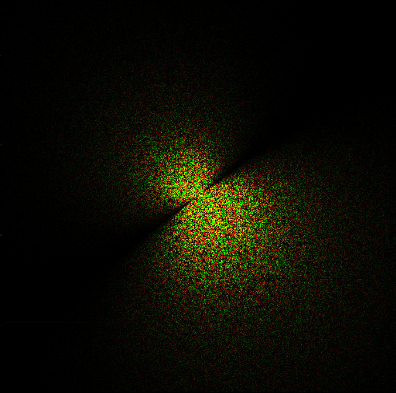
\includegraphics[width=\textwidth]{Images/Other/Fourier_transform}
\end{figure}%\vfil{1em}
\begin{figure}
\centering
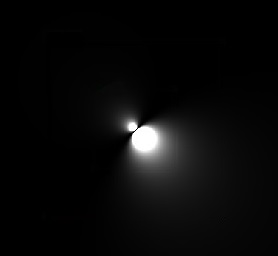
\includegraphics[width=\textwidth]{Images/Other/spectrum_res_increment}
\end{figure}

}

\end{columns}

\end{frame}

\begin{frame}
\frametitle{Fouriersyntes, pseudokod}

\begin{itemize}[<+(1)->]
\item Uppdatering av vattenytan: $\displaystyle H_{n+1}(\vec{k\,}) = e^{i\Delta t\sqrt{gk}}*H_{n}(\vec{k\,})$
\item Pseudokod: \texttt{\\
for all k\_vec in H's domain \{         \\
\ \ \ \ float k = k\_vec.length();      \\
\ \ \ \ float a = dt*sqrt(g*k);         \\
\ \ \ \ H(k\_vec) *= cos(a) + i*sin(a); \\
\}                                      \\
h = Re(invFFT(H));                      \\
}
\end{itemize}


\end{frame}

\begin{frame}
\frametitle{Fouriersyntes, videos}

\begin{itemize}
\item \href{http://www.youtube.com/watch?v=sf6EVn2Zgk4}{MerCUDA, a real time GPU-based ocean simulator}
\item \href{http://www.youtube.com/watch?v=Lj_V5-bTvK0}{Offshore rescue}
\item \href{http://www.youtube.com/watch?v=3YW9WFwD-rI}{Real time stormy ocean 3D}
\item \href{http://www.youtube.com/watch?v=ocHyTiHEphg}{Ship Simulator Extremes Gameplay}
\end{itemize}

\end{frame}